\chapter{Theory}

\section{Furuta's Pendulum}

Rotational inverted pendulum or Furuta’s pendulum composes of two main parts: motor-driven arm, which rotates in the horizontal plane and a pendulum, attached to that arm, which freely rotates in the vertical plane. The system is underactuated and extremely nonlinear due to the gravitational forces and the coupling arising from the Coriolis and centripetal forces. The schematic representation of the pendulum is shown in \ref{furuta}
\begin{figure}[h]
	\centering
	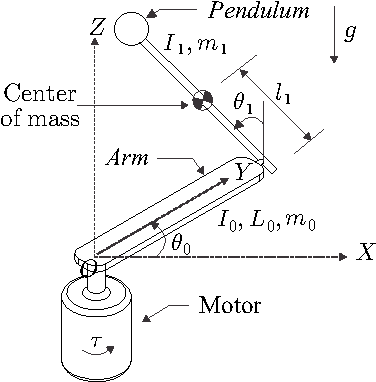
\includegraphics[width=.6\linewidth]{images/furuta}
	\caption{Furuta's Pendulum}
	\label{furuta}
\end{figure}
\newpage
The symbols in the figure indicate the following:
\begin{itemize}
	\item \textbf{$g$} - gravitational acceleration [\si{\metre\per\square\second}]
	\item \textbf{$m_0$} - mass of arm [\si{\kilogram}]
	\item \textbf{$m_1$} - mass of pendulum [\si{\kilogram}]
	\item \textbf{$L_0$} - length of arm [\si{\metre}]
	\item \textbf{$L_1$} - length of pendulum [\si{\metre}]
	\item \textbf{$l_1$} - location of the pendulums center of mass [\si{\metre}]
	\item \textbf{$I_0$} - moment of inertia of arm [\si{\kilogram\per\square\metre}]
	\item \textbf{$I_1$} - moment of inertia of pendulum [\si{\kilogram\per\square\metre}]
	\item \textbf{$\theta_0$} - arm angle [\si{\radian}]
	\item \textbf{$\theta_1$} - pendulum angle [\si{\radian}]
	\item \textbf{$\tau$} - motor torque [\si{\volt}]
\end{itemize}
\subsection{State-Space Representation}
To obtain the state representation of the process we must define our state variables first:
\begin{equation}
	\begin{bmatrix}
	x_1 & x_2 & x_3 & x_4
	\end{bmatrix}^\intercal = 
	\begin{bmatrix}
	\theta_0 & \dot{\theta_0} & \theta_1 & \dot{\theta_1}
	\end{bmatrix}^\intercal
\end{equation}
Control variable:
\begin{equation} u = \tau \end{equation}
Then we can write our state equations:
\begin{subequations}
\begin{equation}\dot{x_1} = \dot{\theta_0} \end{equation}
\begin{equation}\dot{x_2} = \frac{\gamma(\epsilon\dot{\theta_0}^2+\rho)-\delta(\tau+\beta\dot{\theta_1}^2-\sigma\dot{\theta_0}\dot{\theta_1})}{\gamma^2-\alpha\delta}\end{equation}
\begin{equation}\dot{x_3} = \dot{\theta_1}\end{equation}
\begin{equation}\dot{x_4} = \frac{\gamma(\tau+\beta\dot{\theta_1}^2-\sigma\dot{\theta_0}\dot{\theta_1})-\alpha(\epsilon\dot{\theta_0}^2+\rho)}{\gamma^2-\alpha\delta}\end{equation}
\end{subequations}
where
\begin{equation}\alpha = I_0+L_0^2m_1+l_1^2m_1\sin^2\theta_1\end{equation}
\begin{equation}\beta = L_0m_1l_1\sin\theta_1 \end{equation}
\begin{equation}\gamma = L_0m_1l_1\cos\theta_1\end{equation}
\begin{equation}\delta = I_1+l_1^2m_1\end{equation}
\begin{equation}\epsilon = l^2_1m_1\sin\theta_1\cos\theta_1\end{equation}
\begin{equation}\rho = m_1gl_1\sin\theta_1\end{equation}
\begin{equation}\tau = 2l^2_1m_1\sin\theta_1\cos\theta_1\end{equation}
Now these non-linear differential equations we can write in the form of matrices:
\begin{equation}\label{nonlinmodel}
\begin{bmatrix}
\dot{x_1} \\ \dot{x_2} \\ \dot{x_3} \\ \dot{x_4}
\end{bmatrix} = \begin{bmatrix}
\dot{\theta_0}\\
\frac{\gamma(\epsilon\dot{\theta_0}^2+\rho)-\delta(\tau+\beta\dot{\theta_1}^2-\sigma\dot{\theta_0}\dot{\theta_1})}{\gamma^2-\alpha\delta}\\
\dot{\theta_1}\\
 \frac{\gamma(\tau+\beta\dot{\theta_1}^2-\sigma\dot{\theta_0}\dot{\theta_1})-\alpha(\epsilon\dot{\theta_0}^2+\rho)}{\gamma^2-\alpha\delta}
\end{bmatrix}
\end{equation}
As we can see the states derivatives are the functions of the current states and control input. And more importantly, those variables have nonlinear interactions within each state equation. 
\begin{equation}\begin{bmatrix}
\dot{x_1} \\ \dot{x_2} \\ \dot{x_3} \\ \dot{x_4}
\end{bmatrix} = f(x,u) =\begin{bmatrix}f_1(x,u)\\f_2(x,u)\\f_3(x,u)\\f_4(x,u)\end{bmatrix} \end{equation}
So that’s our non-linear dynamic model of the process. But only the NMPC controller is able to operate with such a model.  So, to make that model suitable for LQR and MPC controller we can approximate that non-linear model by a linear model as follows:
\begin{equation}\dot{x} = Ax + Bu\end{equation}
And the constant matrices are derived as:
\begin{equation}
A = \begin{bmatrix}
\frac{\partial f_1(x,u)}{\partial x_1}&\frac{\partial f_1(x,u)}{\partial x_2}&\frac{\partial f_1(x,u)}{\partial x_3}&\frac{\partial f_1(x,u)}{\partial x_4}\\
\frac{\partial f_2(x,u)}{\partial x_1}&\frac{\partial f_2(x,u)}{\partial x_2}&\frac{\partial f_2(x,u)}{\partial x_3}&\frac{\partial f_2(x,u)}{\partial x_4}\\
\frac{\partial f_3(x,u)}{\partial x_1}&\frac{\partial f_3(x,u)}{\partial x_2}&\frac{\partial f_3(x,u)}{\partial x_3}&\frac{\partial f_3(x,u)}{\partial x_4}\\
\frac{\partial f_4(x,u)}{\partial x_1}&\frac{\partial f_4(x,u)}{\partial x_2}&\frac{\partial f_4(x,u)}{\partial x_3}&\frac{\partial f_4(x,u)}{\partial x_4}
\end{bmatrix}, \quad B = \begin{bmatrix}
\frac{\partial f_1(x,u)}{\partial u}\\\frac{\partial f_2(x,u)}{\partial u}\\\frac{\partial f_3(x,u)}{\partial u}\\\frac{\partial f_4(x,u)}{\partial u}
\end{bmatrix}
\end{equation}
And when we compute these derivatives ve obtain linearised model in form of state matrices
\begin{subequations}
	\begin{equation}
		A =\begin{bmatrix}0&1&0&0\\
				0&0&\frac{-gL_0l_1^2m_1^2}{(m_1L_0^2+I_0)(m_1l_1^2+I_1)-L_0^2l_1^2m_1^2}&0\\
				0&0&0&1\\
				0&0&\frac{gl_1m_1(m_1L_0^2+I_0)}{(m_1L_0^2+I_0)(m_1l_1^2+I_1)-L_0^2l_1^2m_1^2}&0
			\end{bmatrix}, 
	\end{equation}
	\begin{equation}
		B=	\begin{bmatrix}
				0\\ 
				\frac{m_1L_1^2+I_1}{(m_1L_0^2+I_0)(m_1l_1^2+I_1)-L_0^2l_1^2m_1^2}\\
				0\\
				\frac{-L_0l_1m_1}{(m_1L_0^2+I_0)(m_1l_1^2+I_1)-L_0^2l_1^2m_1^2}
	\end{bmatrix}
\end{equation}

\begin{equation}C = \begin{bmatrix}0&0&1&0\end{bmatrix}\end{equation}
\begin{equation}D = 0\end{equation}
\end{subequations}
Now those linearized equations of motion would be evaluated at two equilibrium positions: upright and downward. The reason is that at the downward position the system's output, which is the position of the pendulum, has a stable point at “$+\pi$” and “$-\pi$”, while at the upright position system has no stable point.
 
The model, obtained by linearization around the upright operation point, is used for fulfilling the main control objective, which is stabilizing the pendulum at the upright position. The second model is used to simulate process behavior during initial excitation by a Swing-up controller.
\section{Controller Synthesis}
\subsection{MPC  design}
MPC uses a model of the system to make predictions about the system’s future behavior. MPC solves an online optimization algorithm to find the optimal control action that drives the predicted output to the reference. MPC can handle MIMO systems that may have interactions between their inputs and outputs. It can also handle input and output constraints. MPC has preview capability; it can incorporate future reference information into the control problem to improve controller performance. Due to all these properties MPC provides the highest quality of control performance at the moment.
\subsubsection{MPC formulation}
The model predictive control require the discrete-time state space model is expressed as
\begin{subequations}
	\begin{align}	
	x(t+T_s) = Ax(t) + Bu(t)\\
	y(t) = Cx(t) + Du(t)
	\end{align}
\end{subequations}
Thanks to knoledge of that model we can predict the futures states and outputs of the system.\\
Due to the setup of the controlled process, the MPC should be formulated to regulate the states of the system to the origin. And such MPC can be formulated as
\begin{subequations}
	\begin{align}
		\min_{u_0,...,u_{N-1}} &\sum_{k=0}^{N-1} (\left\| Q_xx_{t+k}\right\|_p+\left\|Q_uu_{t+k}\right\|_p)\\
	    \label{eq217b}s.t.\quad&x_{t+k+1} = Ax_{t+k} + Bu_{t+k}\quad \forall k \in \{1,...,N\}\\
		&x_t = x(t)\\
		\label{cst_x}&x_{t+k}\in\mathcal{X}\quad \forall k \in \{1,...,N\}\\
		\label{cst_u}&u_{t+k}\in\mathcal{U}\quad \forall k \in \{1,...,N\}
	\end{align}
\end{subequations}
where $\mathcal{X}$ and $\mathcal{U}$ are polytopic state and input constraints respectively, and defined as
\begin{subequations}
	\begin{align}
	\mathcal{X} &= \{H_xx\leq K_x\}\}\\
	\mathcal{U} &= \{H_uu\leq K_u\}\}
	\end{align}
\end{subequations}
Unfortinatly such formulation is inappropriate for quadratic programming solver, so it has to be reformulated in a form of a quadratic optimisation problem.
\subsubsection{MPC as a QP optimisation problem}
The QP optimisation problem has the following form
\begin{subequations}
	\begin{align}
	\min_{u_0,...,u_{N-1}} & z^\intercal Pz + 2Q^\intercal z + R\\
	\label{cst_qp}s.t.\quad&Hz\leq G\\
	&H_{eq}z = G_{eq}
	\end{align}
\end{subequations}
As the first step the standart MPC cost function should be written in a vector form
\begin{equation}
	\min_{u_0,...,u_{N-1}} X^\intercal\tilde{Q}_xX + U^\intercal\tilde{Q}_u\,U\\
\end{equation}
where $X$ is a vector of predicted states, $U$ is an optimal trajektory of future control inputs and $\tilde{Q}_x$ and $\tilde{Q}_u$ are the matrices of original weight matrices.
\begin{equation}
	X = \begin{bmatrix}
	x_t\\x_{t+1}\\\vdots\\x_{t+N-1}
	\end{bmatrix}
\end{equation}
\begin{equation}
U = \begin{bmatrix}
u_t\\u_{t+1}\\\vdots\\u_{t+N-1}
\end{bmatrix}
\end{equation}
\begin{equation}
\tilde{Q}_x = \begin{bmatrix}
Q_x&0&\cdots&0\\
0&Q_x&\cdots&0\\
\vdots&\vdots&\ddots&\vdots\\
0&0&\cdots&Q_x
\end{bmatrix}
\end{equation}
\begin{equation}
\tilde{Q}_u = \begin{bmatrix}
Q_u&0&\cdots&0\\
0&Q_u&\cdots&0\\
\vdots&\vdots&\ddots&\vdots\\
0&0&\cdots&Q_u
\end{bmatrix}
\end{equation}
At the next step the equality constrain (\ref{eq217b}) should expressed in the vector form. We can achieve that by predicting the states development over the whole prediction horizon.
\begin{equation}
\begin{split}
x_t = x(t)\\
\hat{x}_{k+1} &= Ax_k + Bu_k\\
\hat{x}_{k+2} &= A\hat{x}_{k+1} + Bu_{k+1}\\
&= A^2x_k + ABu_k + Bu_{k+1}\\
\hat{x}_{k+3} &= A\hat{x}_{k+2} + Bu_{k+2}\\
&= A^3x_k + A^2Bu_k + ABu_{k+1} + Bu_{k+2}\\
&\vdots\\
\hat{x}_{k+N} &= A^Nx_k+\sum_{j=k}^{k+N-1}A^jBu_{k+N-j-1}
\end{split}
\end{equation}
Or if we write these equations in a compact form, we obtain
\begin{equation}
	\begin{bmatrix}
	x_t\\\hat{x}_{t+1}\\ \hat{x}_{t+2}\\\vdots\\ \hat{x}_{t+N-1}
	\end{bmatrix} = 
	\begin{bmatrix}I\\A\\A^2\\ \vdots \\ A^{N-1}\end{bmatrix}x(t) + 
	\begin{bmatrix}
	0& 0&\cdots&0&0\\
	B&0&\cdots&0&0\\
	AB&B&\cdots&0&0\\
	\vdots&\vdots&\ddots&\vdots&\vdots\\
	A^{N-2}B&A^{N-3}B&\cdots&B&0\end{bmatrix}
	\begin{bmatrix}u_k\\u_{k+1}\\u_{k+2}\\\vdots\\u_{k+N-1}\end{bmatrix}
\end{equation}
Or in the short form
\begin{equation}\label{eq227}
	X = \tilde{A}x_t + \tilde{B}U
\end{equation}
At this point we can substitute as $X$ in the cost function by (\ref{eq227}). Then we obtain the new objective function
\begin{equation}\label{eq228}
	\min_{u_0,...,u_{N-1}} (\tilde{A}x_t + \tilde{B}U)^\intercal\tilde{Q}_x(\tilde{A}x_t + \tilde{B}U) + U^\intercal\tilde{Q}_u\,U\\
\end{equation}
And when we expand and simplfie (\ref{eq228}) we obtain
\begin{equation}
	U^\intercal(\tilde{B}^\intercal\tilde{Q}_x\tilde{B} + \tilde{Q}_u)U + 2x_t^\intercal\tilde{A}^\intercal\tilde{Q}_x\tilde{B}U + x_t^\intercal\tilde{A}\tilde{Q}_x\tilde{A}x_t
\end{equation}
Where we can cleary see matrices $P$, $Q$ and $R$, which occurs in a standart cost function for the quadratic optimisation.
\begin{subequations}
	\begin{align}
		P &= \tilde{B}^\intercal\tilde{Q}_x\tilde{B} + \tilde{Q}_u\\
		Q &= (2x_t^\intercal\tilde{A}^\intercal\tilde{Q}_x\tilde{B}U)^\intercal\\
		R &= x_t^\intercal\tilde{A}\tilde{Q}_x\tilde{A}x_t
	\end{align}
\end{subequations}
Now only constrains remain. Constrains (\ref{cst_x}) and (\ref{cst_u}) must be reformulated as (\ref{cst_qp}). Those constrains we consider as a upper and lower bounds for the states and control inputs respectively
\begin{subequations}
	\begin{align}
		x_{min} &\leq x_k \leq x_{max} \quad \forall k \in \{1,...,N\}\\
		u_{min} &\leq u_k \leq u_{max} \quad \forall k \in \{1,...,N\}
	\end{align}
\end{subequations}
Now we split and vectorise those constrains
\begin{subequations}
\begin{align}
	X &\leq X_{max}\\
	-X &\leq -X_{min}\\
	U &\leq U_{max}\\
	-U &\leq -U_{min}
\end{align}
\end{subequations}
In the next step we substitute $X$ in the states constrains by a (\ref{eq227}) and express $U$
\begin{subequations}
	\begin{align}
	\tilde{B}\,U &\leq X_{max} - \tilde{A}x_t\\
	-\tilde{B}\,U &\leq -X_{min} + \tilde{A}x_t\\
	U &\leq U_{max}\\
	-U &\leq -U_{min}
	\end{align}
\end{subequations}
Those constrains are in the standart form and by combining them we obtain matrices of inequality constrains $H$ and $G$ for the quadratic optimisation problem
\begin{equation}
	H = \begin{bmatrix}
	\tilde{B}\\
	-\tilde{B}\\
	I\\
	-I\\
	\end{bmatrix}, \quad
	G = \begin{bmatrix}
	X_{max} - \tilde{A}x_t\\
	-X_{min} + \tilde{A}x_t\\
	U_{max}\\
	-U_{min}
	\end{bmatrix}
\end{equation}
At this point, as matrices $R$, $Q$, $R$, $H$ and $G$ are defined, we can implement MPC by using any quadratic programming solver.
\subsection{Energy Shaping controller design}
For initial excitation of the system we use the energy-based swing-up controller. The strategy with this controller is that we increase the amplitude of swings by increasing the energy of the system with every swing. The energy is added by controlling arms movements and depends on the actual energy of the pendulum. The actual energy of the pendulum can be calculated from the actual position of the pendulum and its velocity: 
\begin{equation}
E = \frac{m_1gl_1}{2}((\frac{\dot{\theta_1}}{\omega_0})^2+\cos\theta_1 - 1)
\end{equation}
Than the control law has following form:
\begin{equation}
	u = k_vEsign(\dot{\theta_1}\cos\theta_1)
\end{equation}
Where element $sign(\dot{\theta_1}\cos\theta_1)$ determines direction i which the force will be applied and $k_vE$ is the gain of the controller.







